\section{Introduction}

Simulation is often used to inspect various characteristics of a system.
In the SoOS project\footnote{See \url{http://www.soos-project.eu/} and \cite{soos} for details.} we inspect service-oriented aspects of operating systems.
One part of the project requires to simulate the interactions between software components of an operating system (in the following: OS) and between
OS and application software.

The main issue is: it is in fact not desirable to keep the whole, monolithic, OS kernel on the each core of a multicore machine.
Doing so has detrimental effects on the caches of the individual cores.\cbcomment{citation needed?}
Moving to larger distributed systems, monolithic kernels hinder scalability as the entire internal state has to be synchronized amongst the copies.\cbcomment{I don't think we should say more about S(o)OS or its ideas / concepts in the intro.}
% For example, we could dedicate some cores to an application and some cores to an OS.
% One possible approach to this is the partitioning of the address space. \olcomment{is this so?}
% In a simular manner, if we know that a core is occupied by a particular program, we can move the dynamic libraries, required for some other application to some other core's memory range.
% A further issue is the scalability of the parallel system.

Overcoming the aforementioned limitations of contemporary operating system designs is the motivation for the S(o)OS project \cite{soos}.
The project aims to research OS concepts and specific OS modules, which aid in scalability of the complete software stack (both OS and application) on future many-core systems.
One of the key concepts of S(o)OS is that only those OS modules needed by a application thread, are actually loaded into the (local) memory of a CPU core on which the thread will run.
This execution environment thus differs from contemporary operating systems where every core runs a complete copy of the (monolithic) operating system.

While creating new operating system concepts and regarding their interaction with the programmability of large-scale systems, we found that existing simulation packages do not seem to have the right abstractions for fast design exploration \cite{cotson,omnet}.
The ability to simulate separate components of the OS and of the application was the main goal to develop the OS simulator \soosim \olcomment{cite the WATERS paper if it is accepted until submission}.
\soosim is also available from Hackage.\footnote{Issue \cd{cabal install soosim} to install \soosim. See also:
\url{http://github.com/christiaanb/SoOSiM}.}
The design decisions were:
\begin{itemize}
\item To simulate message passing and shared memories as the main forms of communication between software components.
\item To have global \emph{ticks}, designating an abstract notion of time.
\end{itemize}
However, we additionally required a way to implement \emph{blocking} messaging as a means to provide \emph{synchronization} between components.
In other words, if a blocking message is sent, the sender is waiting for the answer---regardless \emph{when}\cbcomment{when \emph{or} where?} in the sender the message is sent.
% If a blocking message is received, the reviever should suspend its current work and process the message.\olcomment{is this true?}
This means, we required the notion of a suspending computation---\emph{suspendable} at any moment of execution of the simulated component.
In the following we will show that using Haskell \cite{haskell-report} enabled us to implement this property in a nice way.
The contributions of this paper include:
\begin{itemize}
\item A short overview of the SoOS project
\item The description of the embedded domain-specific language (eDSL) used to implement OS components in \soosim.
\item The description of \emph{a} eDSL to describe applications that will run on within a \soosim \emph{simulated} system.
\item The list of Haskell language features, we found particularly useful in this project.
\end{itemize}

The remaining part of this paper is organised as follows.
% Section~\ref{sec:soos-project} gives an overview of the SoOS project and of the role \soosim plays in the project.
Section~\ref{sec:soosim-an-overview} described the structure of the \soosim simulator from the user's perspective.
Section~\ref{sec:dsl} gives an implementation overview of the domain specific language, used to implement \soosim.
Section~\ref{sec:impl-detail} discusses Haskell features from which our implementation especially benefited.
Section~\ref{sec:related-work} covers related work.
Section~\ref{sec:concl-future-work} concludes and gives an outlook for the further research.

% \section{SoOS Project}
% \label{sec:soos-project}
%
% The SoOS project \olcomment{....... } \cite{soos}...
\olcomment{Do we need an overview of the whole project then?}

\section{\soosim: An Overview}
\label{sec:soosim-an-overview}

\paragraph{Basic structure.}
The purpose of \soosim is to provide a platform that allows a developer to observe the interactions between OS modules and application threads.
For this reason the simulated hardware is highly abstract.

In \soosim, the hardware platform is described as a set of nodes.
Each \emph{node} represents a physical computing object: such as a core, complete CPU, memory controller, etc.
Every node has a local memory of potentially infinite size.
The layout and connectivity properties of the nodes are not part of the system description.
If such a level of detail is required it would have to be modelled explicitly by the user.

Each \emph{node} hosts a set of components.
A \emph{component} represents an executable object: such as a thread, application, OS module, etc.
Components communicate with each other either using direct messaging, or through the local memory of a node.
Having both explicit messaging and shared memories, \soosim supports the two well known methods of communication.
Because multiple components can send messages to one component, all component have a message queue.
All components in a simulated system, even those hosted within the same node, are executed concurrently.
The simulator poses no restrictions as to which components can communicate with each other, nor to which node's local memory they can read from and write to.
A user of \soosim would have to model those restrictions explicitly if required.
A schematic overview of an example system can be seen in Figure~\ref{fig:system}.

%\def\svgwidth{\columnwidth}
\begin{figure}
\centering
%\includesvg{system}
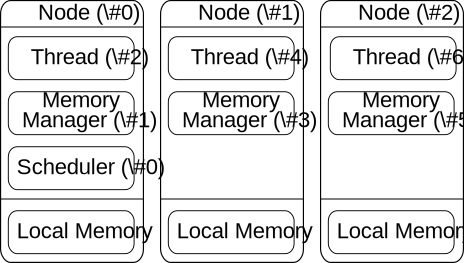
\includegraphics[width=0.7\linewidth]{system}
\caption{System, abstracted.}
\label{fig:system}
\end{figure}

\paragraph{Agility.}
Basic requirements that we would have towards any simulator, include the facilities to straightforwardly simulate the instantiation of application threads and OS modules.
Aside from the fact that the S(o)OS-envisioned system will be dynamic as a result of loading OS modules on-the-fly; large-scale systems also tend to be dynamic in the sense that computing nodes can disappear (failure), or
appear (hot-swap).
Hence, we also require that our simulator facilitates the straightforward creation and destruction of computing elements.
Our current need for a simulator rests mostly in formalizing the S(o)OS concept, and examining the interaction between our envisioned OS modules and the application threads.
As such, being able to extract highly accurate performance figures from a simulated system is not a key requirement.
We do however wish to be able to observe all interactions among application threads and OS modules.
Additionally, we wish to be able to \emph{zoom in} on particular aspects of the behaviour of an application: such as memory access, messaging, etc.

The simulator progresses all components concurrently in one discrete step called a \hs{tick}.
During a \emph{tick}, the simulator passes the content that is at the head of the message queue of each individual component.
If the message queue of a component is empty, a component will be executed with a \emph{null} message.
If desired, a component can inform the simulator that it does not want to receive these \emph{null} messages.
In that case the component will not be executed by the simulator during a \emph{tick}.


\subsection{OS Component Descriptions}

The OS components are also specified in Haskell, each component is modelled as a function.
In case of \soosim, such a function is executed within the context of the simulator, this means: in a \emph{monad}.

Because the function is executed within the monad, it can have \emph{side-effects} such as sending messages to other components, or reading the memory of a local memory.
In addition, the function can be temporarily suspended at (almost) any point in the code.
\soosim needs to be able to suspend the execution of a function so that it may emulate synchronous message passing between components, a subject we will further elaborate later on.

We describe a component as a function that receives a user-defined internal state as its first argument and a value of type \hs{SimEvent} as its second argument.
The result of this function is the internal state.
A value of type \hs{SimEvent} is either message from another component, or a \emph{null} message.
We thus have the following general type signature for a component:
%\numbersoff
\begin{code}
component :: State -> SimEvent -> SimM State
\end{code}

The simulator monad \hs{SimM} is described in Figure~\ref{fig:code-simm}. \olcomment{Move that text block next to here?}
The user-defined internal \hs{State} can be used to store any information that needs to perpetuate across simulator ticks.
\hs{State} should be read as a placeholder for any (user-defined) datatype; there is no actual predefined \hs{State} datatype.

To include a component description in the simulator, the developer will have to create an instance of the \hs{ComponentIface} \emph{type class}.
% A \emph{type class} in Haskell can be compared to an interface
% definition as those known in object-oriented languages.  An
% \emph{instance} of a \emph{type class} is a concrete instantiation
% of such an interface.
%% haskell people know that!
The \hs{ComponentIface} requires the instantiation of the following values to completely define a component:

\begin{itemize}
  \item The initial internal state of the component.
  \item The unique name of the component.
  \item The monadic function describing the behaviour of the component.
\end{itemize}

Note, we are aiming at a high level of abstraction for the behavioural descriptions of our OS modules, where the focus is mainly on the interaction with other OS modules and application threads.


\subsection{Interaction with the simulator}

%% we agreed on not having this figure
% \begin{figure*}
% \centering
% \begin{code}
% createComponent :: Maybe NodeId -> Maybe ComponentId -> String -> SimM ComponentId   -- Nothing is self
%
% -- Synchronously invokes another component
% invoke :: Maybe ComponentId -> ComponentId -> Dynamic -> SimM Dynamic  -- the invocation argument has to be like this
%
% ...
% \end{code}
% \caption{The interaction interface.}
% \label{fig:comp-types}
% \end{figure*}

Components have several functions at their disposal to interact with the simulator and consequently interact with other components.
% We show the types of these functions in Figure~\ref{fig:comp-types}.
The available functions are:

\paragraph{\hs{createComponent}}
Instantiate a new component on a specified node.
\paragraph{\hs{invoke}}
Send a message to another component and wait for the answer.
Whenever a component uses this function it will be temporarily suspended by the simulator.
Several simulator ticks might pass before the response.
Once the response is available the simulator resumes the execution of the calling component.
Having this synchronization obviates the need to specify the behaviour of a component as a finite state machine---a standard approach in the area.
\paragraph{\hs{invokeAsync}}
Send a message to another component and register a handler with the simulator to process the response.
In a contrast to \hs{invoke}, using this function will \emph{not} suspend the execution of the component.
\paragraph{\hs{respond}}
Send a message to another component as a response to an invocation.
\paragraph{\hs{yield}}
Inform the simulator that the component does not want to receive \emph{null} messages.
\paragraph{\hs{readMem}}
Read at a specified address of a node's local memory.
\paragraph{\hs{writeMem}}
Write a new value at a specified address of a node's local memory.
\paragraph{\hs{componentLookup}}
Lookup the unique identifier of a component on a specified node.
Components have two unique identifiers, their global \emph{name} (as specified in the \hs{CompIface} instance), and a \hs{ComponentId} that is a unique number corresponding to a specific instance of a component.
When you want to \emph{invoke} a component, you need to know the unique \hs{ComponentId} of the specific instance.
To give a concrete example, using the system from Figure~\ref{fig:system} as our context: \emph{Thread (\#6)} wants to invoke the instance of the \emph{Memory Manager} that is running on the same Node (\#2).
As \emph{Thread (\#6)} was not involved with the instantiation of that OS module, it has no idea what the specific \hs{ComponentId} of the memory manager on Node \#2 is.
It knows the unique global name of all memory managers, so it can use the \hs{componentLookup} function to find the \hs{Memory Manager} with ID \#5 that is running on Node \#2.

\section{A Domain-specific Language for \soosim}
\label{sec:dsl}
One of the purposes of \soosim is to observe the interaction between application and OS.
We however do not want to \emph{pollute} our application descriptions with with calls to the simulator functions.
Nor do we want to be forced to describe our application in a monadic style.
Additionally, we want to be in control which interactions between OS and application are exactly simulated, without having to change either the descriptions of the OS modules or the application when we want to observe different aspects.

It is for the above reasons that we have chosen to make use of embedded languages for the definitions of our applications.
The idea is to specify an application once in a self-created embedded language, and define different interpretations for the embedded language constructs as the observations of the interaction between application and OS.

Following the \emph{final tagless} \cite{final_tagless_embedding} encoding of embedded languages in Haskell, we use a type class to define the language constructs.
As a running example we demonstrate a mini functional language with mutable references.
A partial specification of the \hs{Symantics} (a pun on \emph{syntax} and \emph{semantics}) type class, defining our \emph{embedded language}, is shown in Figure~\ref{fig:embedded_language_interface}.

\begin{figure}
\centering
\begin{code}
class Symantics repr where
  fun   :: (repr a -> repr b) -> repr (a :-> b)
  app   :: repr (a :-> b) -> repr a -> repr b

  drf   :: repr (Ref a) -> repr a
  (=:)  :: repr (Ref a) -> repr a -> repr Void
\end{code}
\caption{Embedded language, a partial definition.}
\label{fig:embedded_language_interface}
\end{figure}

One interaction we might now want to observe is the applications use of mutable references and the subsequent communication with the memory manager OS module.
For this purpose we create a \hs{newtype} (\hs{RefMemAcc}) wrapping the simulator monad, and define an instance of the \hs{Symantics} type-class for our \hs{newtype}.
Where we would define most of the language constructs to behave like their Haskell counterparts, we define those language constructs dealing with mutable references as invocations of the memory manager (ref Figure~\ref{lst_observing_memory_access}.

\begin{figure}
\centering
\begin{code}
newtype RefMemAcc = RMA SimM

instance Symantics RefMemAcc where

  drf x = RMA $ do
    i     <-- foo x
    mmId  <-- componentLookup "MemoryManager"
    fmap unmashal $ invoke mmId (marshal (Read i))

  x =: y = RMA $ do
    i     <-- foo x
    v     <-- bar y
    mmId  <-- componentLookup "MemoryManager"
    fmap unmashal $ invoke mmId (mashal (Write i v))
\end{code}
\caption{Observing memory access (partial definition).}
\label{lst_observing_memory_access}
\end{figure}

\subsection{Final Tagless}

\olcomment{- Final tagless \cite{final_tagless_embedding}

- Tillmann embedded DSL with type classes
\cite{Hofer:2008:PED:1449913.1449935}

-- move to related work?}

\section{Implementation Details}
\label{sec:impl-detail}

\olcomment{Rename to ``features we used''?}

\subsection{Type classes}

Type classes are naturally used for the eDSL encoding from the previous section. \olcomment{more details on this?}

Beyond this, we use type classes to express many other useful abstractions.
For instance, an \emph{interface} for the component of the OS is a type class.
Thus, each interacting ``building block'' in the simulated software is an instance of that particular type class.
This enables great flexibility, including an option to extend the kinds of simulated objects by third party.

\subsection{Monads}
\olcomment{Merge to OS Component Descriptions? Or: keep!}  
We use a monad called \cd{SimM} to capture the \emph{State} \olcomment{sure?}  of the simulator.
We use \textsf{Control.Monad.Coroutine} express coroutins \cite{coroutines}.
With this concept we capture \olcomment{...}
We use dynamic types for as ``the other side'' of the type classes: we need to communicate heterogeneous types over a typed channel, and there is no option to know all the types-to-transmit at the moment of the channel definition.
\olcomment{this is rather a summary of what we have used, than an introduction to our monad. Move!}

\begin{figure}
\centering
\begin{code*}
type SimMonad =  StateT SimState IO
data SimState = ...

newtype SimM a
  = SimM { runSimM :: Coroutine
      (RequestOrYield Unique Dynamic)
      SimMonad a }
    deriving (Functor, Monad)

data RequestOrYield request response x
  = Request request (response -> x)
  | Yield   x

instance Functor (RequestOrYield x f) where
  fmap f (Request x g) = Request x (f . g)
  fmap f (Yield y)     = Yield (f y)
\end{code*}
\caption{Implementing \cd{SimM}.}
\label{fig:code-simm}
\end{figure}

The implementation of \cd{SimM}, sketched in Figure~\ref{fig:code-simm}, enables us to reach the main implementation goal: the ultimate suspension and resume of the components upon message passing.
To suspend a computation we can now merely write \cd{request componentId}, where the \cd{componentId} is the unique ID of the OS component we are expecting a message from.
The execute a resumeable computation we issue \cd{resume computation}.


\subsection{Coroutines}
As one could infer from Figure~\ref{fig:code-simm}, the implementation makes use of the coroutines in the following way. \olcomment{explain it!}


\section{Related Work}
\label{sec:related-work}

\paragraph{Operating systems and simulators.}
\olcomment{Related work from WATERS paper + more!}
COTSon \cite{cotson} is a full system simulator that allows a developer to execute normal x86 code in a simulated environment.
COTSon is far too detailed for our needs, and does not facilitate the easy exploration of a complete operating system.

OMNeT++ \cite{omnet} is a C++-based discrete event simulator with focus on parallel systems. OMNeT++ is too static for our purposes, it disallows dynamic modules.


\citeauthor{house} describe a basic operating system implementation in Haskell called House \cite{house}.
This work is in a sense dual to ours: we simulate an OS.
\citeauthor{house} modified GHC run-time system to allow code execution on bare metal.
In House, OS modules are executed with the \hs{Hardware} monad, allowing direct interaction with real hardware. 
This approach is comparable with our \hs{Simulator} monad.
However, as we are more concerned with interaction of OS modules, House in not suitable for our purposes:  OS modules in House must be implemented in full detail.

Barrelfish \cite{barrelfish} is an OS in which domain-specific languages are used, amongst other purposes, to define driver interfaces.
These embedded languages are also implemented in Haskell.
The approach used in Barrelfish is however to create parsers for their languages, in a contrast to our embedding approach.


\paragraph{Embedded domain-specific languages.}
For the concept of an eDSL see the papers by \citeauthor{hudak1} \cite{hudak1,hudak2}, the 1998 paper describes pure embedding.
The literature on this topic is quite broad, an overview is presented, \eg by \citeauthor{dsl-survey} \cite{dsl-survey}.

The final tagless embedding of DSLs originates from the seminal paper by \citeauthor{final_tagless_embedding} \cite{final_tagless_embedding}.
\citeauthor{Hofer:2008:PED:1449913.1449935} \cite{Hofer:2008:PED:1449913.1449935} presented a paper that compared to the work by \citeauthor{final_tagless_embedding} \cite{final_tagless_embedding} is more composable, allows subtyping, and is done in Scala \cite{odersky2008programming}.
These two papers have different goals: \citeauthor{final_tagless_embedding} implement DSLs for higher-order languages, while \citeauthor{Hofer:2008:PED:1449913.1449935} focus on the possibility to plug in multiple implementations of a pure embedded DSL.


\section{Conclusions and Future Work}
\label{sec:concl-future-work}

\paragraph{Conclusions.} \olcomment{What have we seen?}
We have presented the efforts, required to implement \soosim, an OS simulator in Haskell.
We note that the techniques more commonly used in the programming language research were highly applicable for our purposes.

We have demonstrated how the utilisation of final tagless eDSL contruction \cite{final_tagless_embedding}, type classes \cite{Hall:1996:TCH:227699.227700}, monads \cite{Wadler:1990:CM:91556.91592}, and coroutines \cite{coroutines} facilitated an abstract and concise implementation of an operating system simulator. 
\olcomment{These techniques belong to the typical repertoire of a programming language designer, but not of an operating systems researcher. --- emphasise somehow, that it is uncommon to use all these for such a task, this this work is cool.}

\paragraph{Real life simulations.}
The major goal of the project is to simulate the behaviour of a real life application and to draw conclusions therefrom.
This work is still ongoing.

\paragraph{Concurrency.}
One aspect of the future work is the concurrent \soosim.
One option is to use Concurrent Haskell \cite{ConcHs}, it provides (concurrent) green threads.
However, it would also require to use software transactional memory \cite{springerlink:10.1007/s004460050028} because of multiple writes to the same data.
Examples of fruitful combinations with other concepts include papers by \citeauthor{Harris:2008:CMT:1378704.1378725} \cite{Harris:2008:CMT:1378704.1378725} and \citeauthor{Bieniusa:2010:BAA:1835698.1835714} \cite{Bieniusa:2010:BAA:1835698.1835714,springerlink:10.1007/978-3-642-25959-3_2}.
Another option would be to use a \emph{parallel} Haskell like Multicore Haskell \cite{marlow:rsm}, \cd{Par} monad \cite{par-monad} or Eden \cite{eden}.
The ``multiple writes'' issue, however, needs some further handling in this case.
A yet further option is to make the coroutine execution concurrent using, \eg actors \cite{Hewitt:1973:UMA:1624775.1624804,sulzmann2008actors}.

% \appendix
% \section{Appendix Title}
%
% This is the text of the appendix, if you need one.

\acks

%Acknowledgments, if needed.
This work was supported by the S(o)OS project, sponsored by the European Commission under FP7-ICT-2009.8.1, Grant Agreement No. 248465.

%%% Local Variables:
%%% mode: latex
%%% TeX-master: "soosim"
%%% End:
